\documentclass{report}

%%%%%%%%%%%%%%%%%%%%%%%%%%%%%%%%%%%%%%%% IMPORTS %%%%%%%%%%%%%%%%%%%%%%%%%%%%%%%%%%%%%%%%
\documentclass[11pt,onesize,a4paper,titlepage]{article}

%%%%%%%%%%%%%%% Formatting %%%%%%%%%%%%%%% 
\usepackage[english]{babel}
\usepackage[utf8]{inputenc}
\usepackage{adjustbox}
\usepackage{geometry} % Margins
\usepackage{sectsty} % Custom Sections

%%%%%%%%%%%%%%% Font %%%%%%%%%%%%%%% 
\usepackage{Archivo}
\usepackage[T1]{fontenc}
\sffamily

%%%%%%%%%%%%%%% Graphics %%%%%%%%%%%%%%% 
\usepackage{fontawesome5} % Icons
\usepackage{graphicx} % Images
\usepackage[most]{tcolorbox} % Color Box
\usepackage{xcolor} % Colors
\usepackage{tikz} % For Drawing Shapes
%%%\usepackage{emoji} % For flags
\tcbuselibrary{breakable}
%%%\usepackage{academicons}

%%%%%%%%%%%%%%% Miscelanous %%%%%%%%%%%%%%% 
\usepackage{lipsum} % Lorem Ipsum
\usepackage{hyperref} % For Hyperlinks

%%%%%%%%%%%%%%% Colors %%%%%%%%%%%%%%% 
\definecolor{title}{HTML}{b5bff5} % Color of the title
\definecolor{bars}{HTML}{889af0} % Color of the title
\definecolor{backdrop}{HTML}{f2f2f2} % Color of the side column
\definecolor{lightgray}{HTML}{dfdfdf} % Color for the skill bars

%%% TU green: #639a00
%%% TU gray: #e6e6e6
%\definecolor{title}{HTML}{639a00} % Color of the title TU
%\definecolor{bars}{HTML}{889af0} % Color of the title TU

% \definecolor{backdrop}{HTML}{f2f2f2} % Color of the side column
\definecolor{backdrop}{HTML}{e6e6e6} % Color of the side column

\definecolor{subtitle}{HTML}{606060} % 


%%%%%%%%%%%%%%% Section Format %%%%%%%%%%%%%%% 
\sectionfont{                     
    \LARGE % Font size
    \sectionrule{0pt}{0pt}{-8pt}{1pt} % Rule under Section name
}

\subsectionfont{
    \Large % Font size
    \fontfamily{phv}\selectfont % Font family
    %\sectionrule{0pt}{0pt}{-8pt}{1pt} % Rule under Subsection name
    \sectionrule{5pt}{0pt}{0pt}{0pt} % Rule under Subsection name
}

%%%%%%%%%%%%%%% Margins and Headers %%%%%%%%%%%%%%%
\geometry{
  a4paper,
  left=7mm,
  right=7mm,
  bottom=10mm,
  top=10mm
}

\pagestyle{empty} % Empty Headers
%%%%%%%%%%%%%%%%%%%%%%%%%%%%%%%%%%%%%%%% MACROS %%%%%%%%%%%%%%%%%%%%%%%%%%%%%%%%%%%%%%%%

%%%%%%%%%%%%%%% Link With an Icon %%%%%%%%%%%%%%% 
\newcommand{\link}[1]{
    \href{#1}{\faIcon{link}}
}

%%%%%%%%%%%%%%% Name Template %%%%%%%%%%%%%%% 
\newcommand{\name}[2]{
    % Name
    \Huge % Font size
    \raggedright \textbf{#1} \par

    \vspace*{0.3cm}
    
    % Profession
    \Large % Font size
    \raggedright #2 \par
    \normalsize \normalfont
}

%%%%%%%%%%%%%%% Contact Details %%%%%%%%%%%%%%%
\newcommand{\info}[2]{
    \faIcon{#2} \hspace{0.2em} #1
}

%%%%%%%%%%%%%%% Email %%%%%%%%%%%%%%%
\newcommand{\email}[1]{
    \info{#1}{envelope}
}

%%%%%%%%%%%%%%% Phone Number %%%%%%%%%%%%%%%
\newcommand{\phone}[1]{
    \info{#1}{mobile-alt}
}

%%%%%%%%%%%%%%% Address %%%%%%%%%%%%%%%
\newcommand{\address}[1]{
    \info{#1}{map-marker-alt}
}

%%%%%%%%%%%%%%% GitHub %%%%%%%%%%%%%%%
\newcommand{\github}[2]{
    \info{\href{#1}{\underline{#2}}}{github}
}

%%%%%%%%%%%%%%% LinkedIn %%%%%%%%%%%%%%%
\newcommand{\linkedin}[2]{
    \info{\href{#1}{\underline{#2}}}{linkedin}
}

%%%%%%%%%%%%%%% ResearchGate %%%%%%%%%%%%%%%
\newcommand{\researchgate}[2]{
    \info{\href{#1}{\underline{#2}}}{researchgate}
}

%%%\newcommand*{\Researchgate}[1]{\sociallink{\researchgatesocialsymbol}{http://www.#1}{#1}}

%%%%%%%%%%%%%%% Website %%%%%%%%%%%%%%%
\newcommand{\website}[1]{
    \info{#1}{link}
}

%%%%%%%%%%%%%%% Draw Skill Bars %%%%%%%%%%%%%%% 
\newcommand{\drawskillbars}[1]{
    \begin{tikzpicture}
        % Draw 5 gray bars
        \foreach \i in {0, 1, 2, 3, 4}{
            \fill[lightgray] (\i * 0.7 + 0.2 *\i,0) rectangle (0.7 + \i * 0.7 + \i * 0.2,0.1);
        }
        
        % Draw number of black bars depending on the skill level
        \foreach \i in {#1}{
            \fill[blue!40] (\i * 0.7 + 0.2 *\i,0) rectangle (0.7 + \i * 0.7 + \i * 0.2,0.1);
            %\fill[title] (\i * 0.7 + 0.2 *\i,0) rectangle (0.7 + \i * 0.7 + \i * 0.2,0.1);
        }
    \end{tikzpicture} \par
}
    
%%%%%%%%%%%%%%% Skills %%%%%%%%%%%%%%%
\newcommand{\skill}[3]{
    % Name of the skill
    \large
    \noindent \hangafter=0
    \adjustbox{valign=t}{\begin{minipage}{0.72\textwidth}
        \large \noindent \hangafter=0
        % Name of the skill
        \textmd{#1} 
        \normalsize \par 
        \vspace{1em}
         % Description
        \noindent \small \color{subtitle} \parbox{1\linewidth}{\textsl{#3}} \par
        \normalsize \par
        \end{minipage}}
    \adjustbox{valign=t}{\begin{minipage}{0.2\textwidth}
        % Skill bars
        \large \hangafter=0
        %\noindent 
        \drawskillbars{#2}
        \end{minipage}}
    \normalsize \par 
    % Skill bars
    %%\drawskillbars{#2}
    %%\vspace{0.5em}
    
    \vspace{1.0em}
    \normalsize \color{black} \par
}

%%%%%%%%%%%%%%% Software %%%%%%%%%%%%%%%
\newcommand{\soft}[2]{
    \adjustbox{valign=t}{\begin{minipage}{0.40\textwidth}
        \large \noindent \hangafter=0
        % Name of the skill
        \textmd{#1} 
        \normalsize \par 
        \vspace{1em}
        \end{minipage}}
    \adjustbox{valign=t}{\begin{minipage}{0.5\textwidth}
        % Skill bars
        \large \noindent \hangafter=0
        \drawskillbars{#2}
        \end{minipage}}
    \normalsize \par 
    \vspace{1em}
}

%%%%%%%%%%%%%%% Personal details %%%%%%%%%%%%%%%
\newcommand{\details}[2]{
    % Name of the language
    \large
    \noindent \hangafter=0 \color{black}
    \adjustbox{valign=t}{\parbox{0.27\linewidth}{#1}}  \adjustbox{valign=t}{\parbox{0.55\linewidth}{#2}} \par
    \vspace{.3em}
    \normalsize \color{black} \par
 }

%%%%%%%%%%%%%%% Language %%%%%%%%%%%%%%%
\newcommand{\lan}[2]{
    % Name of the language
    \large
    \noindent \hangafter=0 \color{black}
    \parbox{0.3\linewidth}{\textmd{#1}}   \color{subtitle} \parbox{0.4\linewidth}{\textsl{#2}} \par
    %\large English \color{subtitle} \textit{Advanced} 
    %\normalsize \par 
    % Knowledge level
    %\noindent \small \color{subtitle} \parbox{1\linewidth}{\textsl{#2}} \par
    \vspace{1.0em}
    \normalsize \color{black} \par
 }

%%%%%%%%%%%%%%% Education %%%%%%%%%%%%%%%
\newcommand{\education}[4]{
    % Name of the studies
    \noindent \large \parbox{.65\linewidth}{\textbf{#1}}
    % Duration in a Box
    \hfill \small
    \tcbox[enhanced,nobeforeafter,box align=base,colback=title,colframe=title,size=fbox,arc=0mm, valign=bottom]{{\textbf{#2}}} \par
    \vspace{0.3em}
    % School Name 
    \normalsize
    \noindent \color{subtitle} \parbox{.9\linewidth}{\textsl{#3}} \par
    % Description
    \normalsize \color{black}
    \vspace*{0.3em}
    \small #4 
    \normalsize \par
    \vspace*{0.5em}
}

%%%%%%%%%%%%%%% Work Experience %%%%%%%%%%%%%%%
\newcommand{\work}[4]{
    % Name of the Job
    \noindent \large \parbox{.65\linewidth}{\textbf{#1}}
    % Duration in a Box 
    \hfill \small
    \tcbox[enhanced,box align=base,nobeforeafter,colback=title,colframe=title,size=fbox,arc=0mm]{\textbf{#2}} \par
    \vspace{0.3em}
    % Name of the Employer
    \noindent \large \color{subtitle} \parbox{.9\linewidth}{\textsl{#3}} \par
    % Description of the job
    \vspace*{0.3em} \color{black}
    \small #4 
    \normalsize \par
}

%%%%%%%%%%%%%%% Teaching %%%%%%%%%%%%%%%
\newcommand{\teaching}[3]{
    % What, Topic and Who/Where/when
    \noindent \adjustbox{valign=t}{\parbox{.99\linewidth}{\text{#1} \text{#2} \textbf{#3}}} 
    \vspace{0.5em}
    \vspace*{1em} 
}

%%%%%%%%%%%%%%% Publications %%%%%%%%%%%%%%%
\newcommand{\publ}[4]{
    % Authors, Title and journal
    \noindent \parbox{.99\linewidth}{\textsl{#3}. \textbf{#1} \textsl{#2} \link{#4}}
    \vspace{0.5em}
    \vspace*{1em} \color{black}
    }

%%%%%%%%%%%%%%% Talks %%%%%%%%%%%%%%%
\newcommand{\talk}[3]{
    % Authors, Title and journal
    \noindent \parbox{.99\linewidth}{\textsl{#3}. \textbf{#1} \textsl{#2}}
    \vspace{0.5em}
    \vspace*{1em} \color{black}
}

%%%%%%%%%%%%%%% Events %%%%%%%%%%%%%%%
\newcommand{\event}[3]{
    \noindent \parbox{.99\linewidth}{\textbf{#1} \textsl{#3} \textsl{#2}}
    \vspace{0.5em}
    \vspace*{1em} \color{black}
}
%---------------------------------------
% BlackBoard Math Fonts :-
%---------------------------------------

%Captital Letters
\newcommand{\bbA}{\mathbb{A}}	\newcommand{\bbB}{\mathbb{B}}
\newcommand{\bbC}{\mathbb{C}}	\newcommand{\bbD}{\mathbb{D}}
\newcommand{\bbE}{\mathbb{E}}	\newcommand{\bbF}{\mathbb{F}}
\newcommand{\bbG}{\mathbb{G}}	\newcommand{\bbH}{\mathbb{H}}
\newcommand{\bbI}{\mathbb{I}}	\newcommand{\bbJ}{\mathbb{J}}
\newcommand{\bbK}{\mathbb{K}}	\newcommand{\bbL}{\mathbb{L}}
\newcommand{\bbM}{\mathbb{M}}	\newcommand{\bbN}{\mathbb{N}}
\newcommand{\bbO}{\mathbb{O}}	\newcommand{\bbP}{\mathbb{P}}
\newcommand{\bbQ}{\mathbb{Q}}	\newcommand{\bbR}{\mathbb{R}}
\newcommand{\bbS}{\mathbb{S}}	\newcommand{\bbT}{\mathbb{T}}
\newcommand{\bbU}{\mathbb{U}}	\newcommand{\bbV}{\mathbb{V}}
\newcommand{\bbW}{\mathbb{W}}	\newcommand{\bbX}{\mathbb{X}}
\newcommand{\bbY}{\mathbb{Y}}	\newcommand{\bbZ}{\mathbb{Z}}

%---------------------------------------
% MathCal Fonts :-
%---------------------------------------

%Captital Letters
\newcommand{\mcA}{\mathcal{A}}	\newcommand{\mcB}{\mathcal{B}}
\newcommand{\mcC}{\mathcal{C}}	\newcommand{\mcD}{\mathcal{D}}
\newcommand{\mcE}{\mathcal{E}}	\newcommand{\mcF}{\mathcal{F}}
\newcommand{\mcG}{\mathcal{G}}	\newcommand{\mcH}{\mathcal{H}}
\newcommand{\mcI}{\mathcal{I}}	\newcommand{\mcJ}{\mathcal{J}}
\newcommand{\mcK}{\mathcal{K}}	\newcommand{\mcL}{\mathcal{L}}
\newcommand{\mcM}{\mathcal{M}}	\newcommand{\mcN}{\mathcal{N}}
\newcommand{\mcO}{\mathcal{O}}	\newcommand{\mcP}{\mathcal{P}}
\newcommand{\mcQ}{\mathcal{Q}}	\newcommand{\mcR}{\mathcal{R}}
\newcommand{\mcS}{\mathcal{S}}	\newcommand{\mcT}{\mathcal{T}}
\newcommand{\mcU}{\mathcal{U}}	\newcommand{\mcV}{\mathcal{V}}
\newcommand{\mcW}{\mathcal{W}}	\newcommand{\mcX}{\mathcal{X}}
\newcommand{\mcY}{\mathcal{Y}}	\newcommand{\mcZ}{\mathcal{Z}}



%---------------------------------------
% Bold Math Fonts :-
%---------------------------------------

%Captital Letters
\newcommand{\bmA}{\boldsymbol{A}}	\newcommand{\bmB}{\boldsymbol{B}}
\newcommand{\bmC}{\boldsymbol{C}}	\newcommand{\bmD}{\boldsymbol{D}}
\newcommand{\bmE}{\boldsymbol{E}}	\newcommand{\bmF}{\boldsymbol{F}}
\newcommand{\bmG}{\boldsymbol{G}}	\newcommand{\bmH}{\boldsymbol{H}}
\newcommand{\bmI}{\boldsymbol{I}}	\newcommand{\bmJ}{\boldsymbol{J}}
\newcommand{\bmK}{\boldsymbol{K}}	\newcommand{\bmL}{\boldsymbol{L}}
\newcommand{\bmM}{\boldsymbol{M}}	\newcommand{\bmN}{\boldsymbol{N}}
\newcommand{\bmO}{\boldsymbol{O}}	\newcommand{\bmP}{\boldsymbol{P}}
\newcommand{\bmQ}{\boldsymbol{Q}}	\newcommand{\bmR}{\boldsymbol{R}}
\newcommand{\bmS}{\boldsymbol{S}}	\newcommand{\bmT}{\boldsymbol{T}}
\newcommand{\bmU}{\boldsymbol{U}}	\newcommand{\bmV}{\boldsymbol{V}}
\newcommand{\bmW}{\boldsymbol{W}}	\newcommand{\bmX}{\boldsymbol{X}}
\newcommand{\bmY}{\boldsymbol{Y}}	\newcommand{\bmZ}{\boldsymbol{Z}}
%Small Letters
\newcommand{\bma}{\boldsymbol{a}}	\newcommand{\bmb}{\boldsymbol{b}}
\newcommand{\bmc}{\boldsymbol{c}}	\newcommand{\bmd}{\boldsymbol{d}}
\newcommand{\bme}{\boldsymbol{e}}	\newcommand{\bmf}{\boldsymbol{f}}
\newcommand{\bmg}{\boldsymbol{g}}	\newcommand{\bmh}{\boldsymbol{h}}
\newcommand{\bmi}{\boldsymbol{i}}	\newcommand{\bmj}{\boldsymbol{j}}
\newcommand{\bmk}{\boldsymbol{k}}	\newcommand{\bml}{\boldsymbol{l}}
\newcommand{\bmm}{\boldsymbol{m}}	\newcommand{\bmn}{\boldsymbol{n}}
\newcommand{\bmo}{\boldsymbol{o}}	\newcommand{\bmp}{\boldsymbol{p}}
\newcommand{\bmq}{\boldsymbol{q}}	\newcommand{\bmr}{\boldsymbol{r}}
\newcommand{\bms}{\boldsymbol{s}}	\newcommand{\bmt}{\boldsymbol{t}}
\newcommand{\bmu}{\boldsymbol{u}}	\newcommand{\bmv}{\boldsymbol{v}}
\newcommand{\bmw}{\boldsymbol{w}}	\newcommand{\bmx}{\boldsymbol{x}}
\newcommand{\bmy}{\boldsymbol{y}}	\newcommand{\bmz}{\boldsymbol{z}}

%---------------------------------------
% Scr Math Fonts :-
%---------------------------------------

\newcommand{\sA}{{\mathscr{A}}}   \newcommand{\sB}{{\mathscr{B}}}
\newcommand{\sC}{{\mathscr{C}}}   \newcommand{\sD}{{\mathscr{D}}}
\newcommand{\sE}{{\mathscr{E}}}   \newcommand{\sF}{{\mathscr{F}}}
\newcommand{\sG}{{\mathscr{G}}}   \newcommand{\sH}{{\mathscr{H}}}
\newcommand{\sI}{{\mathscr{I}}}   \newcommand{\sJ}{{\mathscr{J}}}
\newcommand{\sK}{{\mathscr{K}}}   \newcommand{\sL}{{\mathscr{L}}}
\newcommand{\sM}{{\mathscr{M}}}   \newcommand{\sN}{{\mathscr{N}}}
\newcommand{\sO}{{\mathscr{O}}}   \newcommand{\sP}{{\mathscr{P}}}
\newcommand{\sQ}{{\mathscr{Q}}}   \newcommand{\sR}{{\mathscr{R}}}
\newcommand{\sS}{{\mathscr{S}}}   \newcommand{\sT}{{\mathscr{T}}}
\newcommand{\sU}{{\mathscr{U}}}   \newcommand{\sV}{{\mathscr{V}}}
\newcommand{\sW}{{\mathscr{W}}}   \newcommand{\sX}{{\mathscr{X}}}
\newcommand{\sY}{{\mathscr{Y}}}   \newcommand{\sZ}{{\mathscr{Z}}}


%---------------------------------------
% Math Fraktur Font
%---------------------------------------

%Captital Letters
\newcommand{\mfA}{\mathfrak{A}}	\newcommand{\mfB}{\mathfrak{B}}
\newcommand{\mfC}{\mathfrak{C}}	\newcommand{\mfD}{\mathfrak{D}}
\newcommand{\mfE}{\mathfrak{E}}	\newcommand{\mfF}{\mathfrak{F}}
\newcommand{\mfG}{\mathfrak{G}}	\newcommand{\mfH}{\mathfrak{H}}
\newcommand{\mfI}{\mathfrak{I}}	\newcommand{\mfJ}{\mathfrak{J}}
\newcommand{\mfK}{\mathfrak{K}}	\newcommand{\mfL}{\mathfrak{L}}
\newcommand{\mfM}{\mathfrak{M}}	\newcommand{\mfN}{\mathfrak{N}}
\newcommand{\mfO}{\mathfrak{O}}	\newcommand{\mfP}{\mathfrak{P}}
\newcommand{\mfQ}{\mathfrak{Q}}	\newcommand{\mfR}{\mathfrak{R}}
\newcommand{\mfS}{\mathfrak{S}}	\newcommand{\mfT}{\mathfrak{T}}
\newcommand{\mfU}{\mathfrak{U}}	\newcommand{\mfV}{\mathfrak{V}}
\newcommand{\mfW}{\mathfrak{W}}	\newcommand{\mfX}{\mathfrak{X}}
\newcommand{\mfY}{\mathfrak{Y}}	\newcommand{\mfZ}{\mathfrak{Z}}
%Small Letters
\newcommand{\mfa}{\mathfrak{a}}	\newcommand{\mfb}{\mathfrak{b}}
\newcommand{\mfc}{\mathfrak{c}}	\newcommand{\mfd}{\mathfrak{d}}
\newcommand{\mfe}{\mathfrak{e}}	\newcommand{\mff}{\mathfrak{f}}
\newcommand{\mfg}{\mathfrak{g}}	\newcommand{\mfh}{\mathfrak{h}}
\newcommand{\mfi}{\mathfrak{i}}	\newcommand{\mfj}{\mathfrak{j}}
\newcommand{\mfk}{\mathfrak{k}}	\newcommand{\mfl}{\mathfrak{l}}
\newcommand{\mfm}{\mathfrak{m}}	\newcommand{\mfn}{\mathfrak{n}}
\newcommand{\mfo}{\mathfrak{o}}	\newcommand{\mfp}{\mathfrak{p}}
\newcommand{\mfq}{\mathfrak{q}}	\newcommand{\mfr}{\mathfrak{r}}
\newcommand{\mfs}{\mathfrak{s}}	\newcommand{\mft}{\mathfrak{t}}
\newcommand{\mfu}{\mathfrak{u}}	\newcommand{\mfv}{\mathfrak{v}}
\newcommand{\mfw}{\mathfrak{w}}	\newcommand{\mfx}{\mathfrak{x}}
\newcommand{\mfy}{\mathfrak{y}}	\newcommand{\mfz}{\mathfrak{z}}

%---------------------------------------
% Bar
%---------------------------------------

%Captital Letters
\newcommand{\ovA}{\overline{A}}	\newcommand{\ovB}{\overline{B}}
\newcommand{\ovC}{\overline{C}}	\newcommand{\ovD}{\overline{D}}
\newcommand{\ovE}{\overline{E}}	\newcommand{\ovF}{\overline{F}}
\newcommand{\ovG}{\overline{G}}	\newcommand{\ovH}{\overline{H}}
\newcommand{\ovI}{\overline{I}}	\newcommand{\ovJ}{\overline{J}}
\newcommand{\ovK}{\overline{K}}	\newcommand{\ovL}{\overline{L}}
\newcommand{\ovM}{\overline{M}}	\newcommand{\ovN}{\overline{N}}
\newcommand{\ovO}{\overline{O}}	\newcommand{\ovP}{\overline{P}}
\newcommand{\ovQ}{\overline{Q}}	\newcommand{\ovR}{\overline{R}}
\newcommand{\ovS}{\overline{S}}	\newcommand{\ovT}{\overline{T}}
\newcommand{\ovU}{\overline{U}}	\newcommand{\ovV}{\overline{V}}
\newcommand{\ovW}{\overline{W}}	\newcommand{\ovX}{\overline{X}}
\newcommand{\ovY}{\overline{Y}}	\newcommand{\ovZ}{\overline{Z}}
%Small Letters
\newcommand{\ova}{\overline{a}}	\newcommand{\ovb}{\overline{b}}
\newcommand{\ovc}{\overline{c}}	\newcommand{\ovd}{\overline{d}}
\newcommand{\ove}{\overline{e}}	\newcommand{\ovf}{\overline{f}}
\newcommand{\ovg}{\overline{g}}	\newcommand{\ovh}{\overline{h}}
\newcommand{\ovi}{\overline{i}}	\newcommand{\ovj}{\overline{j}}
\newcommand{\ovk}{\overline{k}}	\newcommand{\ovl}{\overline{l}}
\newcommand{\ovm}{\overline{m}}	\newcommand{\ovn}{\overline{n}}
\newcommand{\ovo}{\overline{o}}	\newcommand{\ovp}{\overline{p}}
\newcommand{\ovq}{\overline{q}}	\newcommand{\ovr}{\overline{r}}
\newcommand{\ovs}{\overline{s}}	\newcommand{\ovt}{\overline{t}}
\newcommand{\ovu}{\overline{u}}	\newcommand{\ovv}{\overline{v}}
\newcommand{\ovw}{\overline{w}}	\newcommand{\ovx}{\overline{x}}
\newcommand{\ovy}{\overline{y}}	\newcommand{\ovz}{\overline{z}}

%---------------------------------------
% Tilde
%---------------------------------------

%Captital Letters
\newcommand{\tdA}{\tilde{A}}	\newcommand{\tdB}{\tilde{B}}
\newcommand{\tdC}{\tilde{C}}	\newcommand{\tdD}{\tilde{D}}
\newcommand{\tdE}{\tilde{E}}	\newcommand{\tdF}{\tilde{F}}
\newcommand{\tdG}{\tilde{G}}	\newcommand{\tdH}{\tilde{H}}
\newcommand{\tdI}{\tilde{I}}	\newcommand{\tdJ}{\tilde{J}}
\newcommand{\tdK}{\tilde{K}}	\newcommand{\tdL}{\tilde{L}}
\newcommand{\tdM}{\tilde{M}}	\newcommand{\tdN}{\tilde{N}}
\newcommand{\tdO}{\tilde{O}}	\newcommand{\tdP}{\tilde{P}}
\newcommand{\tdQ}{\tilde{Q}}	\newcommand{\tdR}{\tilde{R}}
\newcommand{\tdS}{\tilde{S}}	\newcommand{\tdT}{\tilde{T}}
\newcommand{\tdU}{\tilde{U}}	\newcommand{\tdV}{\tilde{V}}
\newcommand{\tdW}{\tilde{W}}	\newcommand{\tdX}{\tilde{X}}
\newcommand{\tdY}{\tilde{Y}}	\newcommand{\tdZ}{\tilde{Z}}
%Small Letters
\newcommand{\tda}{\tilde{a}}	\newcommand{\tdb}{\tilde{b}}
\newcommand{\tdc}{\tilde{c}}	\newcommand{\tdd}{\tilde{d}}
\newcommand{\tde}{\tilde{e}}	\newcommand{\tdf}{\tilde{f}}
\newcommand{\tdg}{\tilde{g}}	\newcommand{\tdh}{\tilde{h}}
\newcommand{\tdi}{\tilde{i}}	\newcommand{\tdj}{\tilde{j}}
\newcommand{\tdk}{\tilde{k}}	\newcommand{\tdl}{\tilde{l}}
\newcommand{\tdm}{\tilde{m}}	\newcommand{\tdn}{\tilde{n}}
\newcommand{\tdo}{\tilde{o}}	\newcommand{\tdp}{\tilde{p}}
\newcommand{\tdq}{\tilde{q}}	\newcommand{\tdr}{\tilde{r}}
\newcommand{\tds}{\tilde{s}}	\newcommand{\tdt}{\tilde{t}}
\newcommand{\tdu}{\tilde{u}}	\newcommand{\tdv}{\tilde{v}}
\newcommand{\tdw}{\tilde{w}}	\newcommand{\tdx}{\tilde{x}}
\newcommand{\tdy}{\tilde{y}}	\newcommand{\tdz}{\tilde{z}}

%---------------------------------------
% Vec
%---------------------------------------

%Captital Letters
\newcommand{\vcA}{\vec{A}}	\newcommand{\vcB}{\vec{B}}
\newcommand{\vcC}{\vec{C}}	\newcommand{\vcD}{\vec{D}}
\newcommand{\vcE}{\vec{E}}	\newcommand{\vcF}{\vec{F}}
\newcommand{\vcG}{\vec{G}}	\newcommand{\vcH}{\vec{H}}
\newcommand{\vcI}{\vec{I}}	\newcommand{\vcJ}{\vec{J}}
\newcommand{\vcK}{\vec{K}}	\newcommand{\vcL}{\vec{L}}
\newcommand{\vcM}{\vec{M}}	\newcommand{\vcN}{\vec{N}}
\newcommand{\vcO}{\vec{O}}	\newcommand{\vcP}{\vec{P}}
\newcommand{\vcQ}{\vec{Q}}	\newcommand{\vcR}{\vec{R}}
\newcommand{\vcS}{\vec{S}}	\newcommand{\vcT}{\vec{T}}
\newcommand{\vcU}{\vec{U}}	\newcommand{\vcV}{\vec{V}}
\newcommand{\vcW}{\vec{W}}	\newcommand{\vcX}{\vec{X}}
\newcommand{\vcY}{\vec{Y}}	\newcommand{\vcZ}{\vec{Z}}
%Small Letters
\newcommand{\vca}{\vec{a}}	\newcommand{\vcb}{\vec{b}}
\newcommand{\vcc}{\vec{c}}	\newcommand{\vcd}{\vec{d}}
\newcommand{\vce}{\vec{e}}	\newcommand{\vcf}{\vec{f}}
\newcommand{\vcg}{\vec{g}}	\newcommand{\vch}{\vec{h}}
\newcommand{\vci}{\vec{i}}	\newcommand{\vcj}{\vec{j}}
\newcommand{\vck}{\vec{k}}	\newcommand{\vcl}{\vec{l}}
\newcommand{\vcm}{\vec{m}}	\newcommand{\vcn}{\vec{n}}
\newcommand{\vco}{\vec{o}}	\newcommand{\vcp}{\vec{p}}
\newcommand{\vcq}{\vec{q}}	\newcommand{\vcr}{\vec{r}}
\newcommand{\vcs}{\vec{s}}	\newcommand{\vct}{\vec{t}}
\newcommand{\vcu}{\vec{u}}	\newcommand{\vcv}{\vec{v}}
\newcommand{\vcw}{\vec{w}}	\newcommand{\vcx}{\vec{x}}
\newcommand{\vcy}{\vec{y}}	\newcommand{\vcz}{\vec{z}}

%---------------------------------------
% Greek Letters:-
%---------------------------------------
\newcommand{\eps}{\epsilon}
\newcommand{\veps}{\varepsilon}
\newcommand{\lm}{\lambda}
\newcommand{\Lm}{\Lambda}
\newcommand{\gm}{\gamma}
\newcommand{\Gm}{\Gamma}
\newcommand{\vph}{\varphi}
\newcommand{\ph}{\phi}
\newcommand{\om}{\omega}
\newcommand{\Om}{\Omega}


\title{\Huge{Analysis 2 Lecture Notes}\\ \hspace{4cm}-- Upendra Kulkarni}
\author{\huge{Soham Chatterjee}}
\date{}

\begin{document}
\maketitle
\newpage% or \cleardoublepage
% \pdfbookmark[<level>]{<title>}{<dest>}
\pagebreak

\vspace*{5cm}

\begin{center}
	\textbf{Abstract}
\end{center}

This is the lecture notes scribed by me. If you find any mistakes in the notes please email me at \url{sohamc@cmi.ac.in}. 

The whole course is taken by Prof. Upendra Kulkarni, online. If you want the lectures then you can find them in \href{https://youtube.com/playlist?list=PL8I7rVYxS9smyQemVlU10yF9F37ZQN38P}{this link}. Sir mainly followed Prof. Pramath Sastry's Notes (\url{https://www.cmi.ac.in/~pramath/teaching.html#ANA2}). You can find all the assignments problems in the following  \href{https://drive.google.com/drive/folders/1dODMladIJ1f4BfMXVxoU5_YkfmWU8v4q?usp=share_link}{drive link}. Through out the course the books we followed is  Principles of Mathematical Analysis by Walter Rudin. 

\pagebreak
\chapter{Constrained Optimizations and Lagrange Multipliers}
\parinf

\textbf{\textit{Example: }}Optimize $f(x,y)y^2-x^2$ subject to the constraint $h(x,y)=x^2+y^2=1$
\parinn

\begin{center}
	\begin{tikzpicture}
		
		\begin{axis}[xmin=-2,xmax=2, ymin=-2, ymax=2,
			restrict x to domain=-10:10, hide axis]% remove crossing lines at t=90 and t=270
			\addplot[red, variable=t,domain=0:360,samples=200] ({sec(t)}, {tan(t)});
			\addplot[blue,variable=t,domain=0:360,samples=200] ({tan(t)}, {sec(t)});
			\addplot[dashed]{x};
			\addplot[dashed]{-x};
			\addplot[variable=t,domain=0:360]  ({cos(t)}, {sin(t)}) ;
		\end{axis}
	\node[text width=7cm, xshift=12cm,yshift=3cm]{\parindent=1cm In other words we want to find extrema of $f|_M$ where $M$ is the level curve for $h$ at level 1 i.e. $M=h^{-1}(1)$
	
Form the way level sets of $f$ interact with $M$, here we see that we have maximum at $(0,\pm 1)$ and minimum at $(\pm 1,0)$

It also appears that the constrained graph and the level curve of the objective function $f$ are $\underset{ \substack{ \downarrow \\ \text{What it means} } }{\text{tangential}}$ to each other

We will define Tangent Space to a level set of a $C^1$ function at a point $p$ on $M$
};
	\end{tikzpicture}
\end{center}
\section{Tangent Space}
\dfn{Tangent Space}{Tangent Space to a hypersurface $M=f^{-1}(c)$ in $\bbR^n$ where $f:(\text{Open }U\subset \bbR^n)\to \bbR$ is a $C^1$ function and $c\in \bbR$ at a point $p\in M$ is a subspace of $\bbR^n$ defined to be $$T_pM=\ker (f'(p))=\{v\in\bbR^n\mid f'(p)(v)=0\}=\{v\in \bbR^n\mid \nabla f(p)\cdot v=0\}$$}
Geometric tangent space considering to our mental image = $T_pM+p=$ Shift $T_pM$ by vector $p$. Likewise define Normal Space to be the set of vectors orthogonal to $T_pM$ i.e. $T_pM^{\perp}$

\begin{center}
	\begin{tikzpicture}
		\draw[domain=-2:2, smooth, variable=\x] plot ({\x}, {\x*\x});
		\draw (-2,0) -- (2,0);
		\draw (0,4) -- (0,-1);
		\draw[red,dashed] (-0.5,-1) -- (1.5,3);
		\draw[blue,dashed] (1,-0.5) -- (-1,0.5);
		\draw[red] (0,-1) -- (2,3);
		\draw[blue] (2,0.5) -- (-1,2);
		\filldraw[red] (1,1) circle (1pt);
		\node[text width=8cm, xshift=8cm,yshift=2cm]{\parindent=1cm 
		Eg. $f(x,y)=y-x^2$, $M=f^{-1}(0)$. $p=(3,9)\in M$. 
		
		Here $f'(p)=\mat{-2x & 1}_{(3,9)}=\mat{-6& 1}$ $$\mat{x \\ y} \mapsto -6x+y$$ $T_pM=\ker(f'(p))=\{ (x,y)\mid y=6x\}=$ \textcolor{red}{red line}. $N_pM= $ line $y=-\frac16 x =$ \textcolor{blue}{blue line}
		
		Geometric tangent space $=T_pM+p$ and geometric normal space $=N_pM+p$
	};
	\end{tikzpicture}
\end{center}
\section{Lagrange Multiplier}
Let $U$ be open in $\bbR^n$. $f:U\to \bbR$ objective function and $h:U\to \bbR$ constraint function. Want to find extrema of $f$ restricted to the level set $M=\{x\in U\mid h(x)=c\}=h^{-1}(c)$ for $c\in\bbR$

$f|_M$ has local maxima at $p\in M$ means for some $W\subset  U$,  $f(p)\geq f(x)\ \forall \ x\in W\cap M$
\dfn{$C^1$ Path and Velocity Vector}{A $C^1$ path centered at $p\in U$ in $U\subset \bbR^n$ is a $C^1$ map $\gm:(-\veps,\veps)\to U$ where $0\mapsto p$. We call $\gm'(0)=$ velocity of $\gm$ at 0}
\thm[lagmult]{Lagrange Multiplier}{
Let $U$ be open in $\bbR^n$. $f:U\to \bbR$, $h:U\to \bbR$. Let $f,h$ are $C^1$ functions. Let $M=h^{-1}(c)$. If $h'(p)\neq 0$ and $f|_M$ has  a local extrema  at $p\in M$  then  $\exs!\lm\in \bbR$ such that $$\nabla f(p)=\lm \nabla h(p)$$
}
\begin{proof}
Consider paths on level set $M=h^{-1}(c)$ i.e. \begin{center}
	\begin{tikzcd}[column sep={3em},/tikz/column 1/.style={column sep=0},/tikz/column 3/.style={column sep=0em}]
	\gm: &  (-\veps,\veps) \arrow[r] \arrow[rdd]&  M &=h^{-1}(c)\\[-8mm]
	 &  & \cap & \\[-8mm]
	 && U \arrow[r, "h"] & \bbR
\end{tikzcd}
\end{center}
Then $h=\gm(t)=c$ $\forall\ t\in (-\veps,\veps)$. Hence by Chain Rule $$h'(p)\gm'(0)=\nabla h(p)\cdot \gm'(0)=0$$ i.e. $\{\text{velocity vectors of all paths }\gm\text{ on }M\text{ centered at }p\}\subset T_pM$\parinf

\textbf{\textit{Key Fact: }}When $h'(p)\neq 0$ we have equality! Proof of this fact uses \hyperref[th:implicit]{Implicit Function Theorem}\parinn

Now let's recall the objective function $f$ and recall that $p$ s assured to be a local max/min. If $gm$ is a $C^1$ curve on $M$ then in particular $f|_{\text{image}(\gm)}$ also has a max/min at $p$. Therefore $$0=(f\circ \gm)'(o)=\nabla f(p)\cdot \gm'(0)$$i.e. $\nabla f$ is orthogonal to velocity vectors to all curves centered at $p$. 

By claim $\nabla f(p)\perp T_pM$, we already  say $\nabla h(p)\perp T_pM$. We know $\nabla h(p)\neq 0$ by assumption. Hence $\exs! \lm$ such that $\nabla f(p)=\lm \nabla h(p)$
\end{proof}

\section{Some Examples for Applications}
\begin{enumerate}[label=(\roman*)]
	\item $f(x,y)=y^2-h^2$ and $h(x,y)=x^2+y^2$, $c=1$. Therefore $M=h^{-1}(1)=$ Unit Circle
	
	Suppose $p=\mat{a\\ b}$ is an extremum of $f|_M$ $$\nabla f(p)=\mat{-2x\\ 2y}_{(a,b)} = \mat{-2a\\ 2b}\qquad \nabla h(p)=\mat{2x\\ 2y}_{(a,b)} = \mat{2a\\ 2b}$$ We know that $\exs ! \lm \in \bbR$ such that $$\mat{-2a\\ 2b}=\lm \mat{2a\\ 2b}$$ This is not possible unless one of $a,b$ os 0. Therefore \begin{center}
		\begin{tabular}{lcl}
			$a=0$ & $\implies $ &$b=\pm 1$ and $\lm=1$\\
			$b=0$ & $\implies$ & $a=\pm 1$ and $\lm=-1$
		\end{tabular}
	\end{center}
\item $f(x,y)=y$ is subject to constraint $h(x,y)=y-g(x)=0$ where $g:\bbR\to \bbR$ is some $C^1$ function. This is equivalent to finding extrema of $y=g(x)$ as in school

Suppose  $p=\mat{a\\ b}$ gives an extremum $$\nabla f(p)=\mat{0\\ 1}= \lm \nabla h(p)=\lm \mat{-g'(a)\\ 1}$$i.e. $1=\lm\implies 0=-\lm g'(a)\implies g'(a)=0$ as expected
\item $f(x,y)=x^2$ subject to $h(x,y)=y=0$ $$\nabla f=\mat{2x\\ 0}=\lm\nabla h=\mat{0\\ 1}\implies \lm =0, x=0$$
\nt{If we instead take $h(x,)=y^2$, then we get $(,xy)=(0,0)$ but $\lm$ arbitrary}
\item $f(x,y)=xy$ subject to $h(x,y)=\frac{x^2}{9}+\frac{y^2}{4}=1$

$$\nabla f=\mat{y\\ x} = \lm \nabla h=\lm \mat{\frac{2x}{9}\\ \frac{y}{2}}$$ Therefore $$y=\frac{2x}{9}\lm, \quad x=\frac{y}{2}\lm, \quad \frac{x^2}{9}+\frac{y^2}{4}=1$$ 

$\lm=\pm 3$. Find extrema. As constraint = ellipse, a compact set, evaluating $f$ as candidates is enough to find max and min.
\item Find the points on the sphere $x^2+y^2+z^2=9$ closest/furthest from $(a,b,c)\to$ arbitrary point in $\bbR^3$

$f(x,y,z)=(x-a)^2+(y-b)^2+(z-c)^2$ and $h(x,y,z)=x^2+y^2+z^2=9$. Complete this and see that geometrically obvious solution emerge 
\end{enumerate}

Next we will prove \hyperref[th:invthm]{Inverse Function Theorem} and \hyperref[th:implicit]{Implicit Function Theorem} and come back to justify the claim. In fact we will then be able to prove the general version of Lagrange Multiplier Method i.e. with multiple constraints

\section{Generalized Lagrange Multiplier}
\thm[genlagmult]{Generalized Lagrange Multiplier}{$U$ open $\subset \bbR^n=\bbR^{d+m}$ want to find extrema of objective function $f:U\to \bbR$ subject to constraint $h=c$ for a $C^1$ function: $U\to \bbR^m$ where $c\in \bbR^m$  i.e. we want to find extreme of $f|_{M=h^{1}(c)}$
}\parinf

\textbf{\textit{Key Assumption: }}$\forall\ x\in M$, $h'(x)$ is surjective i.e. $h'(x):\bbR^{d+m}\to \bbR^m$. (So $\ker(h'(x))$ has $\dim d$. Recall we called $\ker(h'(x))=T_xM$)

Suppose $f|_M$ has a local extremum at $p\in M$ Then $\exs!$ real numbers $\lm_1,\lm_2,\dots,\lm_m$ such that $$\nabla f(p)=\lm_1\nabla h_1(p)+\cdots+\lm_n\nabla h_n(p)$$where $h(p)=\mat{h_1(p) & \cdots & h_m(p)}^T\in \bbR^m$

\parinn
\begin{proof}
	we will show that \begin{enumerate}[label=\bfseries\tiny\protect\circled{\small\arabic*}]
		\item  $\nabla f(p)\perp T_pM$
		\item Any vector $\perp T_pM$ is a linear combination of $\nabla h_i(p)$
	\end{enumerate}
These are the steps. 
\begin{enumerate}[label=\bfseries\tiny\protect\circled{\small\arabic*}]
	\item Let $v\in T_pM=\ker (f'(p))$. By \href{https://drive.google.com/file/d/11OCy_upvhLy8mH0jCKwFbXqzEX3FBT8Z/view?usp=share_link}{HW4 Problem} $v$ can be represented by some curve based at $p$ni.e. we can find a $C^1$ curve $\gm:(-\veps,\veps)\to M\subset U$ where $0\mapsto p$ such that $\gm'(0)=v$. 
	
	As we have an extremum of $f|M$ at $p$ it is also an extreme point for $(-\veps,\veps)\xrightarrow{\gm}M\xrightarrow{f}\bbR$. So by 1-Variable Calculus $(f\circ\gm)'(0)=0$ i.e. $f'(p)\gm'(0)=0$ i.e. $\nabla f(p)\cdot v=0$
	
	\item For every curve $\gm$ as above $h\circ \gm=$ constant. Therefore $h'(p)\gm'(0)=0$ i.e. $\nabla h'(p)\cdot v=0$ $$h'(p)=\mat{ \del{h_1}{x_1}(p)   & \cdots & \del{h_1}{x_n}(p) \\ \vdots & \ddots & \vdots \\ \del{h_m}{x_1}(p)   & \cdots & \del{h_m}{x_n}(p)  }=\mat{\nabla h_1(p)^T \\ \vdots \\ \nabla h_m(p)^T}=\mat{\nabla h_1(p) & \cdots & \nabla h_m(p)}^T$$ So $$\nabla h_1(p)\cdot v=0,\dots , \nabla h_m(p)\cdot v=0$$Therefore $\underset{\substack{ m\text{ linearly} \\ \text{independent} \\ \text{vectors}  }}{\underbrace{\nabla h_i(p)}}\perp \underset{\substack{ \dim n-m \\ =d }}{\underbrace{T_pM}}$. Everything is in $\bbR^n=\bbR{m+d}$. $\therefore (T_pM)^{\perp}$ has $\nabla h_1(p),\dots, \nabla h_m(p)$ as a basis. i.e. \circled{2} is proved
\end{enumerate}
\end{proof}

\chapter{Implicit Function Theorem}
\textbf{Notation: }For $n>m$ let $n=m+d$. Write points of $\bbR^n=\bbR^d\times \bbR^m$ as $(x,y)$ where $x\in \bbR^d,$ $y\in \bbR^m$
\thmc[implicit]{Implicit Function Theorem}{
Let $U$ open in $\bbR^{d+m}$. $\Phi:U\to \bbR^m$ is a $C^1$ map such that $\Phi'(p)$ is surjective (which means columns of the $m\times (d+m)$ matrix of $\Phi'(p)$ span $\bbR^m$). WLOG suppose the last $m$ columns of $\Phi'(p) $ are linearly independent and hence span $\bbR^m$ i.e. the $m\times m$ matrix ``$\lt.\deld{\Phi}{y}\rt|_p=\mat{D_{d+1}\Phi(p) & \cdots & D_{d+m}\Phi(p)} $" is invertible. Then \begin{enumerate}
	\item $\exs$ a neighorhood $W$ of $a$ in $\bbR^d$ and a unique $C^1$ map $W\xrightarrow{f}\bbR^m$ such that $\begin{rcases}
		f(a)=b, (x,f(x))\in U\ \forall \ x\in W\text{ and}\\
		\Phi(x,f(x))=c\ \forall \ x\in W
	\end{rcases}$ i.e. $f$ is an implicit solution to the equation $\Phi(x,y)=c$
\item One can calculate $f'(x)$ by ``Implicit Differentiation"
\end{enumerate}
}
To understand this, first examine two cases:
\begin{itemize}
	\item When $\Phi$ is a linear map given by a matrix $A$. Here we are solving the equation $A\mat{x\\ y}=c$
	\item $d=m=1$ i.e. $n=2$ $\Phi(x,y)=x^2+y^2-1$, solving $\Phi(x,y)=0=c$. When $\lt.\deld{\Phi}{y}\rt|_{p=(a,b)}\neq 0$ we can locally solve for $y$ in terms of $x$ near $p$. $$D\Phi=\lt.\mat{\del{\Phi}{x} & \del{\Phi}{y}}\rt|_{(a,b)}=\mat{2a & 2b}$$ $2b=0$ at $(\pm 1,0)$
\end{itemize}
\begin{proof}
	We will choose $W$ later. Define \begin{center}
		\begin{tikzcd}
			U \arrow[r, "\psi"] & \bbR^{d+m}\\
			(x,y)\arrow[r, maps to] & (x, \Phi(x,y))
		\end{tikzcd}
	\end{center}
Note $\psi'$ has the matrix $\mat{I & O\\ \del{\Phi}{x} & \del{\Phi}{y}}$. This is nonsingular in a neighborhood of $p$. So by \hyperref[th:invthm]{Inverse Function Theorem} $\psi$ is invertible with $C^1$ inverse in a neighborhood $V$ of $p$
\begin{center}
	\begin{tikzcd}
		V \arrow[r] & \psi(V) \arrow[l]\\[-8mm]
		(a,b)\arrow[r, maps to] & (a,c)\\[-8mm]
		(x,y)\arrow[r, maps to] & (x,\Phi(x,y))\\[-8mm]
		(u,\alpha(u,v)) & (u,v) \arrow[l, maps to]
	\end{tikzcd}
\end{center}Definition of $\alpha(u,v)$ defined on $\psi(V)$. This tells us $\alpha(a,c)=b$. Whenever $\Phi(x,y)=c$ i.e. $$(x,y)\xrightarrow{\Phi}(x,c)\xrightarrow{\psi^{-1}}(x,\alpha(x,c))=(x,y)$$ i.e. $y=\alpha(x,c)$ and $\Phi(x,\alpha(x,c))=c$

So we are forced to define $f(x)=\alpha(x,c)$. But what should be the domain of this function $f$ i.e. what should we take $W$ to be. 

\begin{center}
	$(a,c)\in \psi(V)$ is open $\supset$ $\lt( \text{\begin{tabular}{c}
		open ball $W$ \\ around $a$ in $\bbR^d$
	\end{tabular}} \rt)\times \{c\} $
\end{center}

Now for any $x\in W$ we know $(x,c)\in \psi(V)$ i.e. $(x,\alpha(x,c))\in V$ so we define $f:W\to \bbR^m$ where $f(x)=\alpha(x,c)$ and we have derived the function. Now $\phi^{-1}$ is $C^1$ and $\alpha$ is component of $\phi^{-1}$ so all components of $\phi^{-1}$ is also $C^1$. hence $f$ is $C^1$

Uniqueness of $f$ is not true in general for arbitrary $W$. $\Phi(x,y)=x^2+y^2,\ c=1$. In $W=W_1\sqcup W_2$ $$f(x)=\begin{cases}
	\sqrt{1-x^2} & x\in W_1 \qquad[\text{is forced}]\\
	\sqrt{1-x^2} \text{ or }-\sqrt{1-x^2} & x\in W_2
\end{cases}$$. We have choice for $f$ on $W_2$. 

\textbf{If $W$ is connected, $f$ will be unique}. Eg. take $W$ to be a ball.  Suppose $g$ is another solution to $\Phi(x,y)=c$ i.e. $\Phi(x,g(x))=c$ for $x\in W$ and $g(a)=b$. Then consider the set $S=\{x\in W\mid f(x)=g(x)\}$. Show that this set is both closed (easy $S=(f-g)^{-1}(0)$) and open. 


Calculate derivative of $f$ using the fact that $\psi\circ \psi^{-1}=$ Identity and Chain Rule.
\end{proof}
\ex{Application of Implicit Function Theorem}{
\begin{enumerate}[label=(\roman*)]
	\item Linear map $\Phi:\bbR^{d+m}\to \bbR^m$ given by matrix $A$. Given $A\mat{a\\ b}=c$. Want to solve $A\mat{x\\ y}=c$
	
	$A=[P \mid Q]$ where $P$ is $m\times d$ and $Q$ is $m\times m$ and $Q$ is invertible. i.e. \begin{multline*}
		[P\mid Q]\mat{x\\ y}=c\iff [Q^{-1}P\mid I]\mat{x\\ y}=Q^{-1}c\iff Q^{-1}Px+y=Q^{-1}c\\
		\iff y=Q^{-1}c-Q^{-1}Px
	\end{multline*}
\item We can solve for $y$ in terms of $x$ near any $(a,b)$ on the unit circle when $\lt.\deld{\Phi}{y}\rt|_{(a,b)}\neq 0$. [This is mate when $b\neq 0$ i.e. at all points except $(\pm 1,0)$]. $$\lt.D\Phi\rt|_{(a,b)}=\mat{2a& 2b}$$ We can see directly 

\begin{center}
	$\begin{rcases}
		\text{when }b>0 & y=\sqrt{1-x^2}\\
		\text{when }b<0 & y=-\sqrt{1-x^2}
	\end{rcases}$ near (a,b) in fact $\forall\ x\in (-1,1)$
\end{center}
Similarly we can solve for $x$ in terms of $y$ when $\lt.\deld{\Phi}{x}\rt|_{(a,b)}=2a\neq 0$ This is true when $a\neq 0$
\end{enumerate}

}
\pagebreak
\textbf{\textit{Remark: }} Implicit Function Theorem gives a sufficient condition to be able to locally solve a system of linear equations \begin{center}
	$\begin{rcases}
		\Phi_1(x_1,\dots,x_d,y_1,\dots,y_m)=c_1\\
		\Phi_2(x_1,\dots,x_d,y_1,\dots,y_m)=c_1\\
		\qquad\vdots \qquad\qquad \vdots \qquad\qquad \vdots\\
		\Phi_m(x_1,\dots,x_d,y_1,\dots,y_m)=c_1
	\end{rcases}$\begin{tabular}{l}
	for $y_i$'s in terms of $x_i$'s \\
	locally near a given solution\\
	$y=b$ and $x=a$
\end{tabular}
\end{center}

\nt{
The condition of invertibility of submatrix of $\Phi$ is not necessary. Eg. $\Phi(x,y)=y-x^3$ near $(0,0)$ $$\lt.D\Phi\rt|_{(0,0)}=\lt. \mat{-3x^2 & 1}\rt|_{(0,0)}=\mat{0,1} \qquad \lt.\deld{\Phi}{x}\rt|{(0,0)}=0$$ but still we can solve for $x$ in terms of $y$: $x=\sqrt[3]{y}$ 
}

\end{document}
